%!TEX root = ../graduate-work.tex

\section{Верхние и нижние суммы интеграла Римана}

Для того чтобы строго определить класс интегрируемых функций в смысле Римана, используем
верхние и нижние суммы.

\begin{figure}[h]
	\center{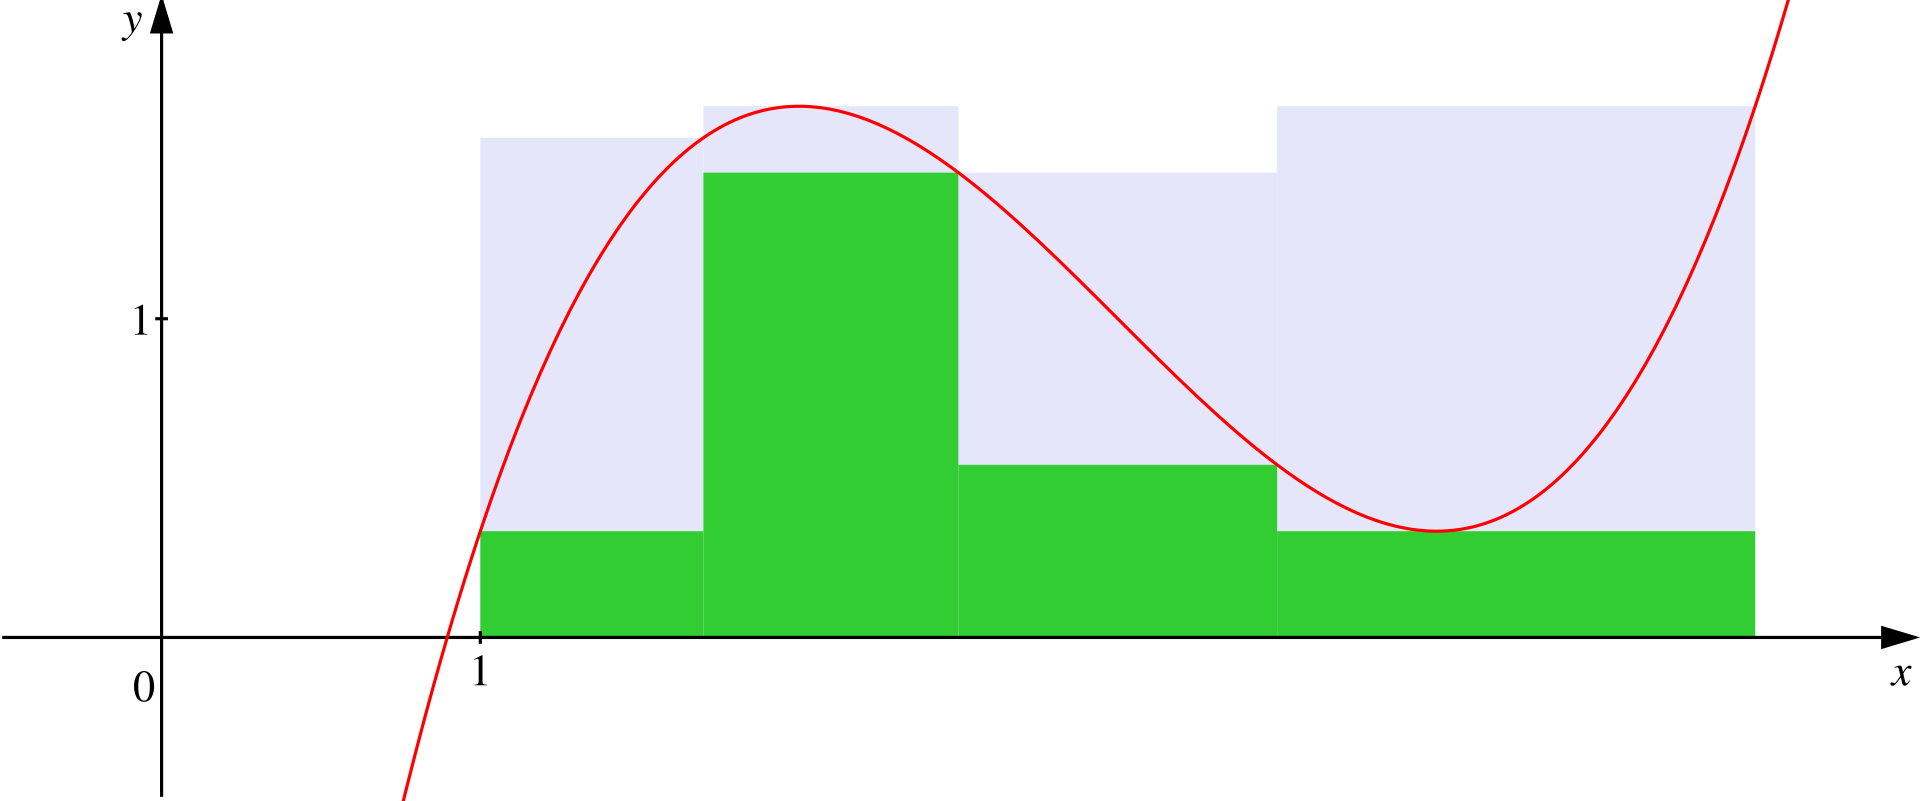
\includegraphics[width=1\linewidth]{upperlower}}
	\caption{Нижняя (зеленая) и верхняя (серая) суммы Дарбу на 4 отрезках разбиения}
	%\label{ris:image}
\end{figure}

\subsection*{Разбиение интервала}

Пусть дана функция \( f(x) \), определённая на отрезке \( [a, b] \). Разбиение
интервала \( [a, b] \) состоит из последовательности точек \( a = x_0 < x_1 <
\dots < x_n = b \), которое делит этот интервал на \( n \) подынтервалов:

\[ \Delta x_i = x_i - x_{i-1}, \quad i = 1, 2, \dots, n.  \]

Каждому подынтервалу \( [x_{i-1}, x_i] \) соответствует несколько значений
функции \( f(x) \) в его пределах.

\subsection{Нижняя сумма Римана}

Нижняя сумма Римана \( L(P, f) \) для разбиения \( P = \{x_0, x_1, \dots, x_n\}
\) и функции \( f(x) \) определяется как сумма произведений длины каждого
подынтервала на инфимум функции \( f(x) \) на этом подынтервале. То есть для
каждого \( i \)-го подынтервала \( [x_{i-1}, x_i] \) выбирается точка, в
которой функция \( f(x) \) принимает минимальное значение:

\[ L(P, f) = \sum_{i=1}^{n} \inf_{x \in [x_{i-1}, x_i]} f(x) \Delta x_i.  \]

Интуитивно, нижняя сумма Римана представляет собой сумму площадей
прямоугольников, где высоты прямоугольников определяются минимальными
значениями функции на каждом подынтервале.

\subsection{Верхняя сумма Римана}

Верхняя сумма Римана \( U(P, f) \) для разбиения \( P \) и функции \( f(x) \)
определяется как сумма произведений длины каждого подынтервала на супремум
функции \( f(x) \) на этом подынтервале. То есть для каждого \( i \)-го
подынтервала \( [x_{i-1}, x_i] \) выбирается точка, в которой функция \( f(x)
\) принимает максимальное значение:

\[ U(P, f) = \sum_{i=1}^{n} \sup_{x \in [x_{i-1}, x_i]} f(x) \Delta x_i.  \]

Таким образом, верхняя сумма Римана представляет собой сумму площадей
прямоугольников, где высоты прямоугольников определяются максимальными
значениями функции на каждом подынтервале.

\subsection{Основное свойство верхних и нижних сумм}

Верхняя и нижняя суммы \( U(P, f) \) и \( L(P, f) \) всегда удовлетворяют
неравенству:

\[ L(P, f) \leq \int_a^b f(x) \, dx \leq U(P, f), \]

где \( \int_a^b f(x) \, dx \) — это значение интеграла Римана, если оно
существует. Таким образом, нижняя и верхняя суммы дают <<ограничения>> на
значение интеграла, и если эти суммы сходятся друг к другу при бесконечно
тонком разбиении, то интеграл Римана существует.

\section{Класс интегрируемых по Риману функций}

Интеграл Римана применяется только к определённому классу функций, которые
называются интегрируемыми по Риману. Эти функции обладают рядом характеристик,
которые позволяют корректно вычислить их интегралы на отрезке \( [a, b] \). В
данной главе рассматриваются основные свойства и критерии для функций,
интегрируемых по Риману.


\subsection{Условия интегрируемости по Риману}

Для того чтобы функция \( f(x) \) была интегрируемой по Риману на отрезке \(
[a, b] \), она должна удовлетворять следующим основным условиям:

\begin{itemize} \item \textbf{Ограниченность.} Функция \( f(x) \) должна быть
			ограниченной на интервале \( [a, b] \). То есть, существует
			такая константа \( M \), что для всех \( x \in [a, b] \)
			выполняется неравенство \( |f(x)| \leq M \).
    
		\item \textbf{Наличие конечного числа разрывов.} Функция \( f(x) \)
			может иметь на интервале \( [a, b] \) разрывы, однако их должно
			быть конечное количество. Если функция имеет бесконечно много
			разрывов, то её интеграл по Риману не существует. Это означает,
			что функция должна быть непрерывной, за исключением конечного
числа разрывов.  \end{itemize}

Примером функции, не интегрируемой по Риману, является функция Дирихле на
интервале \( [0, 1] \), которая принимает значение 1 для рациональных чисел \(
x \) и 0 для иррациональных чисел. Эта функция имеет несчётное число разрывов
на интервале, и её интеграл не существует.

\subsection{Классы интегрируемых функций}

Класс интегрируемых по Риману функций включает в себя множество типов функций,
среди которых выделяются:

\begin{itemize} \item \textbf{Непрерывные функции.} Все функции, которые
			непрерывны на отрезке \( [a, b] \), интегрируемы по Риману. Это
			связано с тем, что непрерывность функции на замкнутом отрезке
			гарантирует, что функция ограничена и не имеет разрывов.
    
		\item \textbf{Функции с конечным числом разрывов.} Функции, имеющие
			конечное количество разрывов на отрезке \( [a, b] \), также
			являются интегрируемыми по Риману. Важно, что эти разрывы не
			могут быть "слишком большими" (например, функции с бесконечными
			разрывами или с бесконечно большим скачком значений не
			интегрируемы).
    
		\item \textbf{Простейшие полиномы и рациональные функции.} Полиномы и
			рациональные функции, ограниченные на интервале, всегда
			интегрируемы по Риману, так как они непрерывны на данном
			интервале.
    
		\item \textbf{Монотонные функции.} Монотонные функции на отрезке \(
			[a, b] \) всегда интегрируемы по Риману, поскольку они
			ограничены и имеют не более конечного числа разрывов.
\end{itemize}

\subsection{Критерий с использованием верхних и нижних сумм}

Функция \( f(x) \) интегрируема по Риману на интервале \( [a, b] \), если и
только если для любого \( \epsilon > 0 \) существует такое разбиение \( P \),
что разница между верхней и нижней суммами будет меньше \( \epsilon \), то
есть:

\[ U(P, f) - L(P, f) < \epsilon.  \]

Это условие гарантирует, что функция можно аппроксимировать с точностью до \(
\epsilon \) с помощью верхних и нижних сумм, и, следовательно, существует
интеграл Римана функции на данном интервале.

\section{Заключение}

Интеграл Римана сыграл ключевую роль в развитии математического анализа,
предоставив чёткую формализацию вычисления площадей, объёмов и других величин.
Его введение стало важной вехой в истории математики, и несмотря на
существование обобщений, интеграл Римана остаётся
одним из основополагающих понятий в математическом анализе. Его применение
охватывает множество областей математики, физики и инженерии.





